\documentclass[a4paper]{article}
\usepackage[utf8]{inputenc}
\usepackage[spanish, es-tabla]{babel}

\usepackage{amsmath}
\usepackage{amsfonts}
\usepackage{amssymb}

\usepackage{float}
\usepackage{graphicx}
\usepackage{subcaption}
\captionsetup{compatibility=false}

\usepackage{multirow}
\setlength{\doublerulesep}{\arrayrulewidth}

\usepackage{array}
\newcolumntype{C}[1]{>{\centering\let\newline\\\arraybackslash\hspace{0pt}}m{#1}}

\usepackage[american]{circuitikz}

\usepackage{fancyhdr}

\usepackage{units} 

\pagestyle{fancy}
\fancyhf{}
\lhead{22.01 Teoría de Circuitos}
\rhead{Mechoulam, Lambertucci, Rodriguez, Londero}
\rfoot{Página \thepage}
\begin{document}


%%%%%%%%%%%%%%%%%%%%%%%%%%%%%%%%%%%
\subsection{Introducción.}
El \textbf{Gyrator} es un componente electrónico inicialmente propuesto como el quinto componente lineal y pasivo luego del resistor, capacitor, inductor y transformador ideal. Fue propuesto en 1948 por Bernard D. H. Tellegen el componente acopla la la corriente en un puerto con la tensión en el otro y viceversa. Siendo caracterizado por un cuadripolo con parametros impedancia:
$$ Z= \left(\begin{matrix}0&-R\\R&0\end{matrix}\right) $$
Donde R sería la resistencia interna del Gyrator.

\begin{figure}[H]	
	\centering
	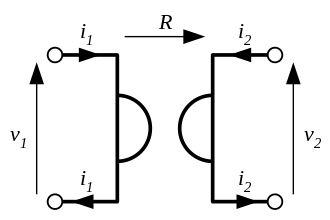
\includegraphics[width=0.7\textwidth]{ImagenesEj2/gyratorsimb.png}
	\caption{Simbolo eléctrico del Gyrator.}
	\label{fig:gyrsimb}
\end{figure}
Realmente es implementado utilizando opamps, y uno de los usos mas populares es para la inversión de impedancias, permitiendo simular un inductor utilizando otros componentes.La configuración generalmente utilizada es la siguiente:
\begin{figure}[H]	
	\centering
	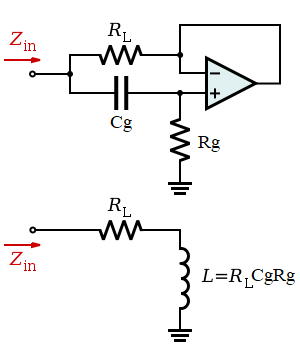
\includegraphics[width=0.5\textwidth]{ImagenesEj2/gyrop.png}
	\caption{Equivalente del circuito Gyrator.}
	\label{fig:gyrop}
\end{figure}

%%%%%%%%%%%%%%%%%%%%%%%%%%%%%%%%%%%%%%%%%
\subsection{Calculo analítico.}
Utilizando el circuito de la figura (\ref{fig:gyrop}) se plantearon las siguientes ecuaciones:
\begin{align}   V_{Out} = V^- \label{eq:1}\end{align}
\begin{align} V_{Out} = A(s) \cdot (V^+-V^-)\label{eq:2}\end{align}
\begin{align} A(s)= \frac{A_0}{1+\frac{s}{\omega'}}\end{align}
\begin{align} I_{In}=\frac{V_{In}-V^-}{R_L}+\frac{V^+}{R_g}\end{align}
\begin{align} V^+=V_{In}\cdot \frac{R_g}{R_g+\frac{1}{sC_g}} \end{align}
primero observaremos que en utilizando (\ref{eq:1}) y (\ref{eq:2}) se llega a que 
\begin{align}V^- =V^+ \cdot \frac{A(s)}{A(s)+1} = V^+ \cdot \frac{A_0}{A_0+1+\frac{s}{\omega'}} \approx V^+ \cdot \frac{1}{1+\frac{s}{GBP}} \label{eq:desp}   \end{align}
Donde GBP es un parámetro propio del operacional y suele ser del orden de los MHz. Por lo tanto este termino sería desprecianle siempre que el rango de frecuencias en los cuales se trabaje sea menor a 50kHz
, teniendo en cuenta esa aproximacion se pueden llegar a las siguientes expresiones:
\begin{align}H(s)= \frac{R_g}{R_g+\frac{1}{sC_g}} \end{align}


\begin{align}Z_{In}=\frac{R_LR_gC_gs+R_L}{sC_gR_L+1}\underset{C_gR_Ls << 1}{\approx}R_gC_gR_L \cdot s + R_g 
\label{eq:Zintrans}
\end{align}

Bajo estos supuestos se puede considerar la impedancia de entrada como una bobina con 
\begin{align}  L=R_gC_gR_L  \ \ \ \ \ \  R_L=r_{coil} \label{eq:basicL1}\end{align}
\flushleft
%%%%%%%%%%%%%%%%%%%%%%%%%%%%%%%%%%%%%%
\subsection{Gyrator vs Inductor}
Hablamos de la impedancia de entrada pero tambien es conveniente preguntarse, porque es necesario suplantar a los inductores con circuitos que se comporten de manera similar.
Los inductores ocupan un gran tamaño respecto a el resto de los componentes que pueden ser integrados para reducir aun mas su tamaño, una desventaja del uso del gyrator, es que su rango operativo en el cual se comporta como inductancia no es muy extenso. Tambien otro factor a tener en cuenta es la desviación estandar respecto al valor nominal de la inductancia, mientras que con el gyrator dado a que los componentes que lo integran son mas precisos el inductor emulado también lo será.

%%%%%%%%%%%%%%%%%%%%%%%%%%%%%%%%%%%%%%%%%%
\subsection{Impedancia de entrada.}
\label{section:zin}
Dado a que la caracteristica mas atractiva del gyrator es que su impedancia de entrada, bajo ciertas hipotesis, se comporta como un inductor se procedió a medirla y se contrasto con una simulación de \textbf{LTSpice} de la impedancia de entrada de un hyrator y la impedancia de entrada de una bobina, también simulada.

\begin{figure}[H]	
	\centering
	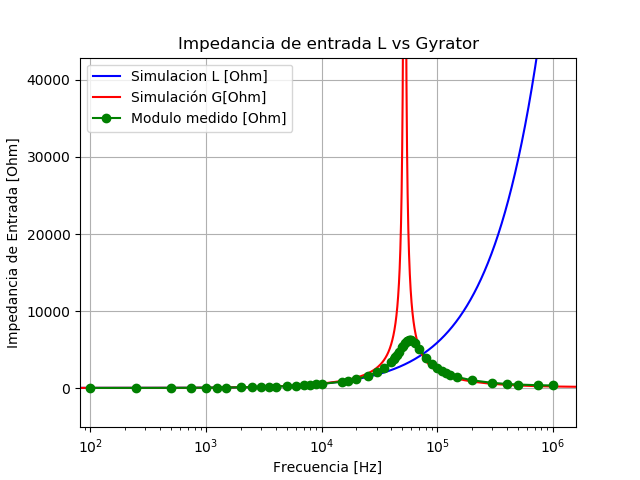
\includegraphics[width=\textwidth]{ImagenesEj2/ZinG.png}
	\caption{Impedancia de entrada del Gyrator.}
	\label{fig:ZinG}
\end{figure}
Puede notarse que el pico el cual presenta el Gyrator simulado no se compara con el medido, esto se atribuye a una posible resonancia que se de en la simulación la cual no se da en el circuito real. Otra cosa a notar es que el gyrator tiene un comportamiento similar a el de una bobina en un rango de frecuencias de 0 ~40 kHz
También se midió la fase obteniendo el siguiente gráfico.
\begin{figure}[H]	
	\centering
	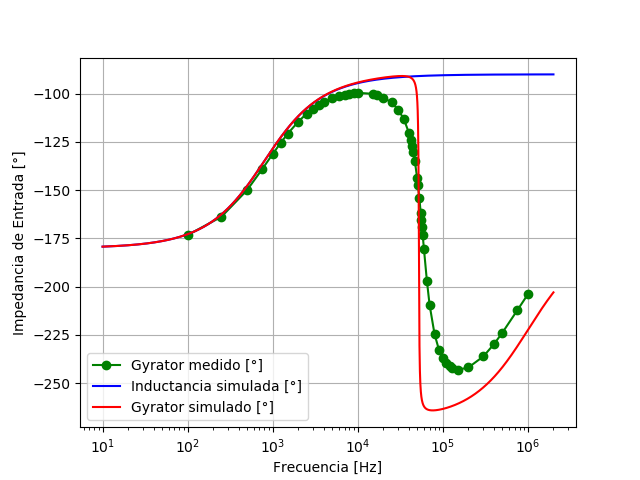
\includegraphics[width=\textwidth]{ImagenesEj2/ZinGp.png}
	\caption{Impedancia de entrada del Gyrator fase.}
	\label{fig:ZinG}
\end{figure}
 Aquí tambien se puede notar la similtud entre las señales hasta aproximadamente 40 kHz, tambien que el cambio de fase en el gyrator medido no es tan brusco comparado  con el simulado.
Finalmente considerando las ultimas mediciones, el rango operativo en el cual se va  a trabajar con el Gyrator será desde 1Hz~40/50 kHz.
%%%%%%%%%%%%%%%%%%%%%%%%%%%%%%%%%%%%%%%
\subsection{Elección operacional.}
El operacional que se eligió fue un operqacion \textbf{TL-084} dado a su $GBP \approx 3MHz$, sus pequeñas corrientes de Bias $I_B \approx 30pA$, su slew-rate $SR \approx 13 \frac{V}{\mu s}$, cuenta con una gran impedancia de entrada, $ r_i \approx 1T \Omega $ y que cuenta con 4 operacionales, la cual es una cualidad notable dado que solamente se podrá utilizar 1 integrado.

%%%%%%%%%%%%%%%%%%%%%%%%%%%%%%%%%%%%%%
 \flushleft
\subsection{Filtros de segundo orden.}
Los filtros a implemetar en este trabajo serán filtros de segundo orden siendo estos Low-Pass, High-Pass, Band-Pass y Band-Reject. Y tendran las siguientes especificaciones de diseño:
\begin{table}[H]
\begin{center}
\begin{tabular}{|c|c|c|c|}
\hline
\textbf{Tipo de Filtro} & \textbf{$f_p$ [Hz]} & \textbf{$f_a$ [Hz]} & \textbf{$f_c$ [Hz]} \\ \hline
\textbf{LP}             & 1000                & 3500                & \textbf{-}          \\ \hline
\textbf{HP}             & 10500               & 3000                & \textbf{-}          \\ \hline
\textbf{BP}             & -                   & -                   & 2000                \\ \hline
\textbf{BR}             & -                   & -                   & 3000                \\ \hline
\end{tabular}
\caption{Tabla de especificaciones.}
\label{tab:specs}
\end{center}
\end{table}
Para el caso de LP que tenga ganancia unitaria para la continua que tenga una ganancia mayor a -3dB para frecuencias menores a $f_p$ y menor a -10dB para frecuencais mayores a $f_a$. Para el HP se desea que tenga ganancia unitaria para valores de $f$ muy grandes, que tenga una ganancia mayor a -3dB para frecuencias mayores a $f_p$ y menor a -10dB para frecuencais menores a $f_a$
Algunos parametros que vale la pena recordar de filtros de segundo orden son:
\begin{table}[H]
\begin{center}
\begin{tabular}{c|cl}
$\omega_0$: & Frecuencia de corte del sistema en [$\frac{rad}{s}$] & =$\frac{1}{\sqrt{LC}}$         \\
$\xi$:      & Factor de Amortiguamiento del sistema.               & =$\frac{R\sqrt{C}}{2\sqrt{L}}$ \\
Q:          & Selectividad del sistema                             & =$\frac{1}{2\xi}$             
\end{tabular}
\end{center}
\caption{Parametros útiles.}
\label{tab:utils}
\end{table}


%%%%%%%%%%%%%%%%%%%%%%%%%%%%%%%%%%%%%%%%%%%%
\subsection{High Pass.}
\subsubsection{Circuito utilizando inductor.}
El circuito propuesto para realizar un filtro pasa altos clasicamente es el siguiente:

\begin{figure}[H]
\begin{center}
\begin{circuitikz}
	\node [](v2){};
	\draw (v2) node[label=left:$V_{In}$]{} to[short, o-] ++ (0.5,0) to[R, l = $R$]++ (1.5,0) to[C, l = $C$] ++ (2,0) to[open] ++(0,-2) node[ground](gnd){};
	\draw (gnd) to[L, l_= $L$] ++(0,2);
	\draw (v2) to[open] ++(4,0) to[short, -o] ++(1,0) node[label=right:$V_o$](){};
	\end{circuitikz}
	\caption{Filtro High-Pass básico.}
	\label{fig:basHP}
\end{center}
\end{figure}

Para este circuito es sumamente facil obtener la transferencia, basta con plantear un divisor resistivo, con lo cual se llega a:
\begin{align} 
H(s)=\frac{s^2LC+s\cdot r_{coil}C}{s^2LC+s\cdot(R+r_{coil})C+1}
\label{eq:HPL}
 \end{align}

\subsubsection{Circuito utilizando Gyrator.}
Para la implementación de este filtro utilizando un Gyrator dado a que este usualmente esta referenciado a tierra  se optó por el siguiente diseño:
\begin{figure}[H]	
	\centering
	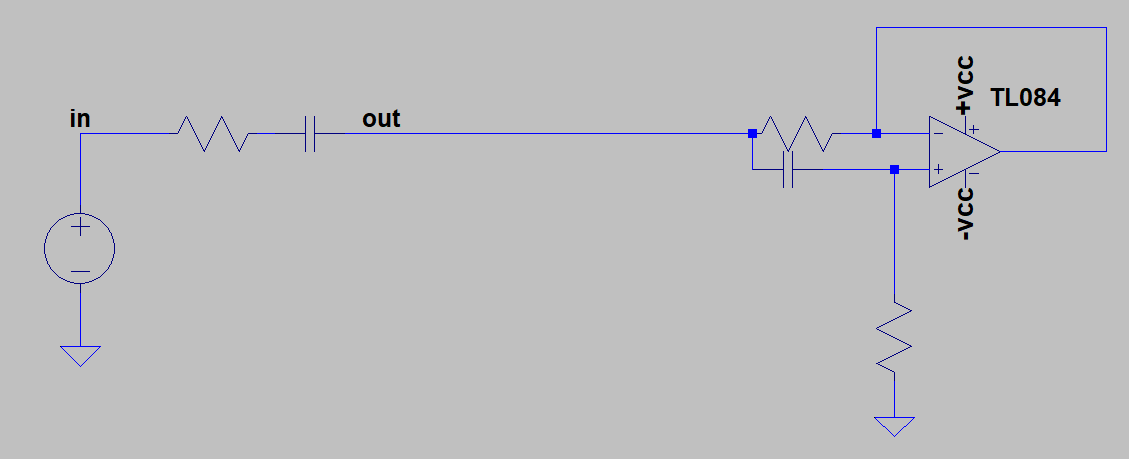
\includegraphics[width=0.7\textwidth]{ImagenesEj2/gyrHP.PNG}
	\caption{Filtro High-Pass implementado con Gyrator.}
	\label{fig:gyrHP}
\end{figure}



Utilizando las siguientes ecuaciones se puede llegar a la expresión de la transferencia:
\begin{align}V^- = V_{o'}\end{align}
\begin{align}V_{o'} = A(s)\cdot (V^+-V^-)\end{align}
\begin{align}\frac{V_o-V_i}{R+\frac{1}{sC}} = \frac{V^+-V_o}{R_L}+(V^+-V_o)\cdot sC_g\end{align}
\begin{align}\frac{-V^+}{R_g}=(V^+-V_o)\cdot sC_g\end{align}
%\begin{align}\end{align}
\begin{align} H(s) = \frac{C R_L s \left(C_g R_g s + 1\right)}{C C_g R R_L s^{2} + C C_g R_g R_L s^{2} + C R s + C R_L s + C_g R_L s + 1}\label{eq:transgyrHP}\end{align}\footnote{Teniendo en cuenta que se despreció el término (\ref{eq:desp}) de (\ref{eq:transgyrHP})}
Luego teniendo en cuenta (\ref{eq:basicL1}) y tomando que
\begin{align} C_gR_LRC<<LC \implies R<<R_g \end{align}
La transferencia  se puede expresar como:
 \begin{align} H(s) = \frac{LC\cdot s^2+Cr_{coil}\cdot s}{s^2 \cdot (LC)+s\cdot C(R+r_{coil})+1}\label{eq:transgyrHPfinal} 
\end{align}
Vale la pena destacar que (\ref{eq:HPL}) y (\ref{eq:transgyrHPfinal}) son iguales.
Es de utilidad recordar las aproximiaciones utilizadas hasta ahora:
\begin{align}  \frac{1}{1+\frac{s}{GBP}}\approx 1  \ \ \ R<<R_g \ \ \ C_gR_Ls << 1 \label{eq:basicL2}\end{align}
\subsubsection{Comparación de modelos.}
Se simuló en \textbf{LTSpice} ambos filtros, siendo estos el implemetnado con gyrator y el implementado con un inductor, obteniendo como era esperado una gran coincidencia en las frecuencias bajas y medias, y finalmente difiriendo en las altas como se ve a continuación:
\begin{figure}[H]	
	\centering
	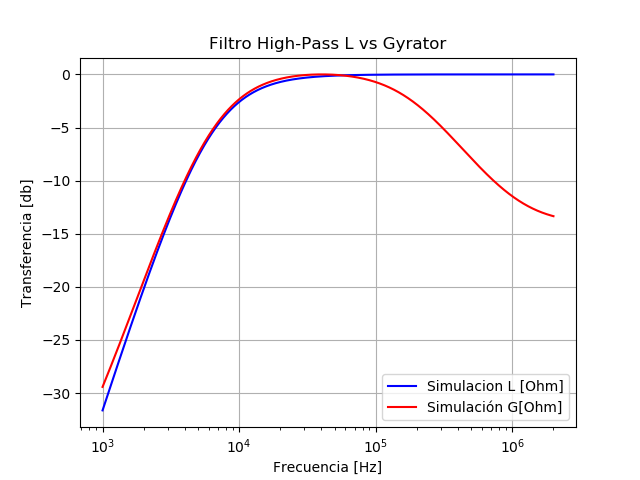
\includegraphics[width=0.7\textwidth]{ImagenesEj2/simHP.PNG}
	\caption{Comparación de modelos Gyrator e Inductor.}
	\label{fig:gyrInd}
\end{figure}
\begin{figure}[H]	
	\centering
	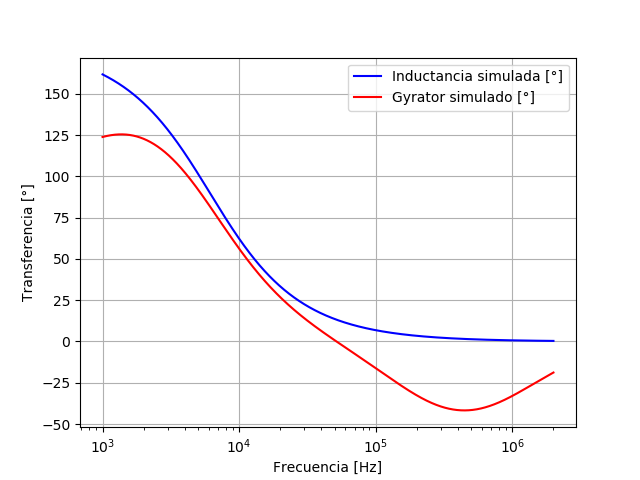
\includegraphics[width=0.7\textwidth]{ImagenesEj2/simHPP.PNG}
	\caption{Comparación de modelos Gyrator e Inductor Fase.}
	\label{fig:gyrIndP}
\end{figure}
Es de interés mencionar que debido a la resistencia interna de la bobina y su análogo de $R_L$ ofrecen un termino lineal en el numerador de la transferencia, este cero introducido es el culpabla de que a las bajas frecuencias la pendiente correspondiente a un sistema de primer orden. Tambien es observable que a partir de una frecuencia, $f_d \approx 1kHz $, la pendiente aumenta a la de un sistema de segundo orden, tal como es deseado.
%%
\subsubsection{Elección de componentes.}
Se eligieron los componentes teniendo en cuenta la tabla (\ref{tab:specs}) para la cual el filtro debe cumplir esas especificaciones.
Lo primero que se decidió fue fijar la impedancia de salida del Gyrator siendo esta de $L \approx 10mH $ y $r_{coil} \approx 51\Omega $, para esto se tomaron los siguientes valores: $R_L = 51\Omega \ R_g = 200k\Omega \ C_g = 1nF$
A partir de esto se decidio una frecuencia de corte de  para que cumpla las especificaciones $f_c =6.1kHz $. Esto define un valor de capacitor $C \approx 68nF$ y finalmente dado a que no debe amplificar para ninguna frecuencia se eligió un valor de R tal que no haya sobrepico\footnote{Cabe aclarar que el valor de $\xi$ para el cual comienza a haber sobrepico es de 0.707} teniendo un valor de $\xi \approx 0.98 $ con $R \approx 750 $
Vale la pena notar que las aproximaciones que se expresaron en (\ref{eq:basicL2}) siguen vigentes. En este caso se tienen los siguientes valores:
\begin{align}  R<<R_g \implies  \frac{R_g}{R}=  267 \ \ \ \ C_gR_L << 1 \implies C_gR_L=5.1 \cdot 10^{-8} \end{align}

%%
\subsubsection{Respuesta en frecuencia.}
Se midió la respuesta en frencuencia del filtro pasa altos, se simuló en \textbf{LTSpice}  tanto el comportamiento con gyrator como el de un inductor. Obteniendo las siguientes gráficas:
\begin{figure}[H]	
	\centering
	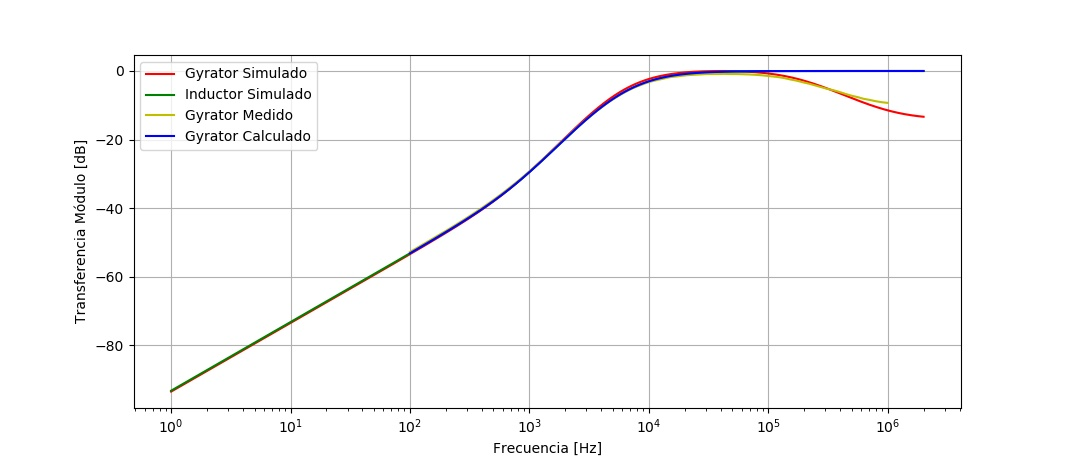
\includegraphics[width=\textwidth]{ImagenesEj2/bodehp.jpg}
	\caption{Diagrama BODE High-Pass Amplitud.}
	\label{fig:bodehp}
\end{figure}
\begin{figure}[H]	
	\centering
	
\includegraphics[width=\textwidth]{ImagenesEj2/bodehpp.jpg}
	\caption{Diagrama BODE High-Pass Fase.}
	\label{fig:bodehpp}
\end{figure}
Se puede observar que...
\subsubsection{Analisis de resultados.}
El mayor interés fue puesto en que el circuito cumpla con las especificaciones dadas en la tabla (\ref{tab:specs})
Obteniendo las siguientes mediciones:


En la figura (\ref{fig:fahp}) se puede observar como para frecuencias a partir de 3kHz la atenuación es mayor a 14dB.
\begin{figure}[H]	
	\centering
	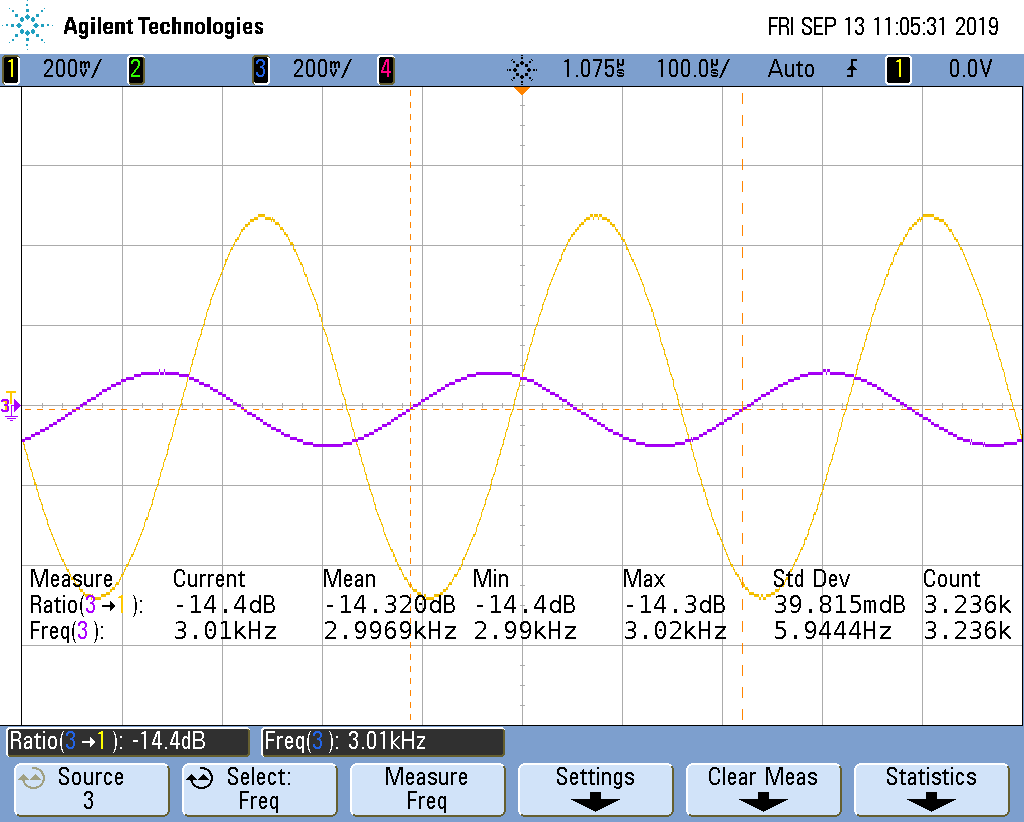
\includegraphics[width=\textwidth]{ImagenesEj2/MedicionesGrilla/fa_hp.png}
	\caption{Frecuencia de atenuación.}
	\label{fig:fahp}
\end{figure}

En la figura (\ref{fig:fphp}) se puede observar como para frecuencias a partir de 10.5kHz, la atenuación es menor a 3dB si bien, es muy próxima.

\begin{figure}[H]	
	\centering
	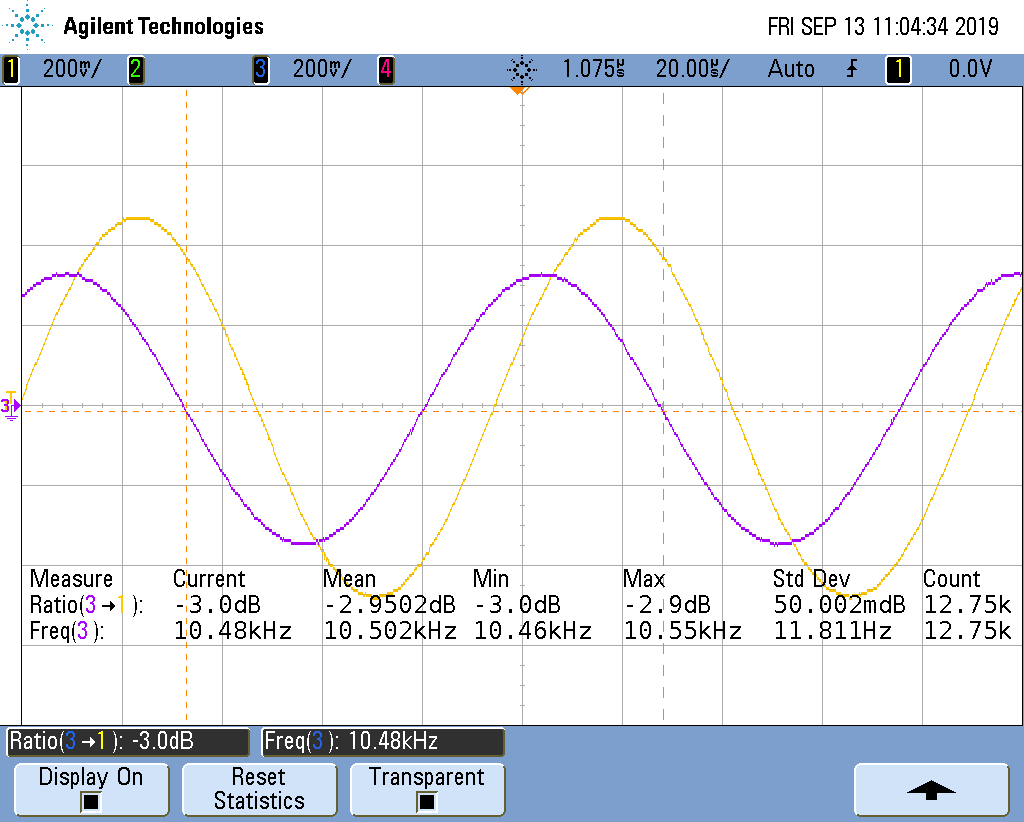
\includegraphics[width=\textwidth]{ImagenesEj2/MedicionesGrilla/fp_hp.png}
	\caption{Frecuencia de paso.}
	\label{fig:fphp}
\end{figure}

\newpage
%%%%%%%%%%%%%%%%%%%%%%%%%%%%%%%%%%%%%%%%%%%%
\subsection{Low Pass.}
\subsubsection{Circuito utilizando inductor.}
El circuito propuesto para realizar un filtro pasa bajos clasicamente es el siguiente:

\begin{figure}[H]
\begin{center}
\begin{circuitikz}
	\node [](v2){};
	\draw (v2) node[label=left:$V_{In}$]{} to[short, o-] ++ (0.5,0) to[R, l = $R$]++ (1.5,0) to[L, l = $L$] ++ (2,0) to[open] ++(0,-2) node[ground](gnd){};
	\draw (gnd) to[C, l_= $C$] ++(0,2);
	\draw (v2) to[open] ++(4,0) to[short, -o] ++(1,0) node[label=right:$V_o$](){};
	\end{circuitikz}
	\caption{Filtro Low-Pass básico.}
	\label{fig:basLP}
\end{center}
\end{figure}
Obteniendo la transferencia del circuito se obtiene:
\begin{align}
H(s)=\frac{1}{s^2\cdot LC+s\cdot C(R+r_{coil})+1}
\label{eq:LPL}
\end{align}
La cual verifica ser un pasabajos.
\subsubsection{Circuito utilizando Gyrator.}
El gyrator tiene la particularidad de que debe estar referenciado a tierra para funcionar como tal, en este caso lo utilizaremos "flotando" para realizar el filtro pasa bajos.La idea que impulsó este diseño fue que el comportamiento de bobina del circuito de la figura (\ref{fig:gyrop}) es visto por el circuito gracias a la impedancia de entrada. En este caso se pensará la R y C como la carga, y se calculó la impedancia de salida del siguiente circuito:

\begin{figure}[H]	
	\centering
	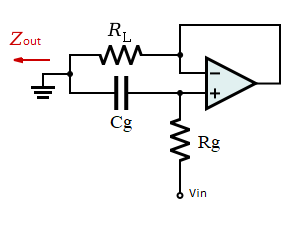
\includegraphics[width=0.7\textwidth]{ImagenesEj2/gyrfloat.png}
	\caption{Gyrator referenciada a la fuente.}
	\label{fig:gyrfloat}
\end{figure}
Para el cual el primer paso será pasivar la fuente y quedará referenciado a masa.De esta manera, el cálculo será análogo al de la sección (\ref{section:zin}) . Por lo cual la impedancia de salida del circuito, conectandole una carga de R y C en serie, proporciona un circuito final, análogo al de la figura (\ref{fig:basLP})
El circuito propuesto fue el siguiente:
\begin{figure}[H]	
	\centering
	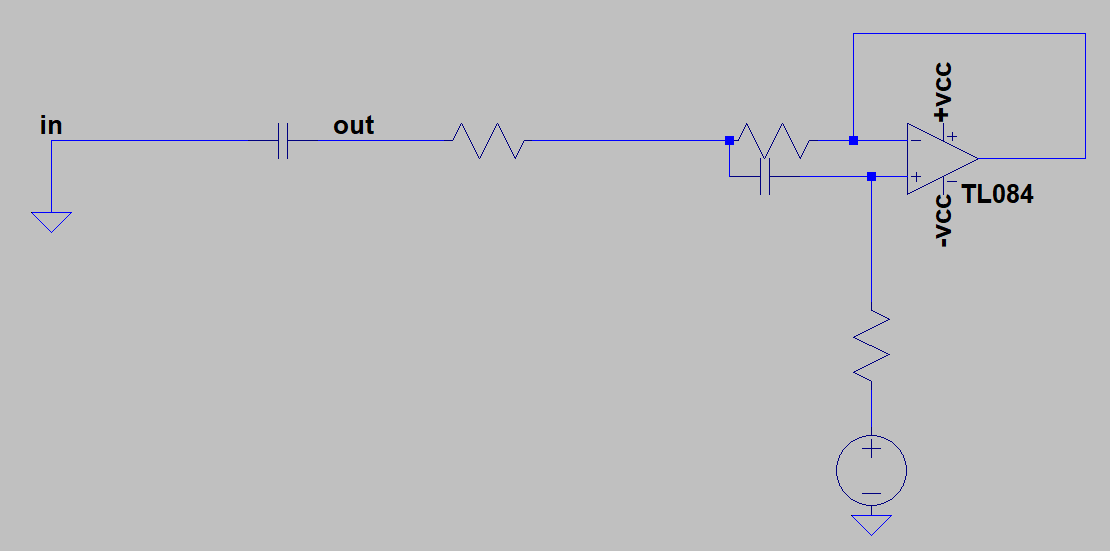
\includegraphics[width=0.7\textwidth]{ImagenesEj2/gyrLP.PNG}
	\caption{Filtro Low-Pass implementado con Gyrator.}
	\label{fig:gyrLP}
\end{figure}

Utilizando las siguientes ecuaciones se puede llegar a la expresión de la transferencia:
\begin{align}V^- = V_{o'}\end{align}
\begin{align}V_{o'} = A(s)\cdot (V^+-V^-)\end{align}
\begin{align}\frac{V_{In}-V^+}{R_g}=(V^+-V_n)\cdot s C_g\end{align}
\begin{align}V_{out}\cdot s C=\frac{V_{n}-V_{out}}{R}\end{align}
\begin{align}\frac{V_{n}-V_{out}}{R}=\frac{V^--V_n}{R_L} +(V^+-V_n)\cdot s C_g\end{align}
%\begin{align}\end{align}
Operando se obtiene:
\begin{equation} H(s)= \frac{\left(C_g R_L s + 1\right)}{C C_g R R_L s^{2} + C C_g R_g R_L s^{2} + C R s + C R_L s + C_g R_L s + 1}
\end{equation}
Utilizando (\ref{eq:basicL1}) y (\ref{eq:basicL2}) se llega a que:
\begin{equation} H(s)= \frac{1}{C L s^{2} + s\cdot C (R+r_{coil}) + 1}
\label{eq:LPG}
\end{equation}
Vale la pena destacar que (\ref{eq:LPL}) y (\ref{eq:LPG}) son iguales y que es un filtro de segundo orden.
%%
\subsubsection{Diseños alternativos.}
Previo a la desición de utilizar el diseño de la figura (\ref{fig:gyrLP}) se idearon otras alternativas. Una fue utilizar una salida diferencial sobre el capacitor, una mejora sobre este último era utilizar un restador para que esta salida diferencial quede referenciada a tierra. Otra alternativa encontrada fue la utilizacion de 2 gyrators para formar un  frequency-dependent negative resistance (FDNR) para realizar el filtro; este diseño finalmente fue desechado dado a que para este ultimo se necesitarían 2 operacionales, y dado la limitacion en el integrado se optó por mantener simple el diseño e implementar el diseño final.
%%
\subsubsection{Comparación de modelos.}
Se simuló en \textbf{LTSpice} ambos filtros, siendo estos el implemetnado con gyrator y el implementado con un inductor, obteniendo como era esperado una gran coincidencia en las frecuencias bajas y medias, y finalmente difiriendo en las altas como se ve a continuación:
\begin{figure}[H]	
	\centering
	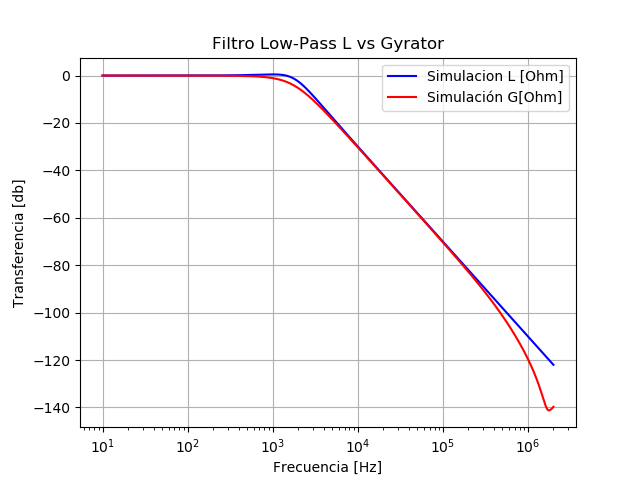
\includegraphics[width=0.7\textwidth]{ImagenesEj2/simLP.PNG}
	\caption{Comparación de modelos Gyrator e Inductor.}
	\label{fig:gyrIndL}
\end{figure}
\begin{figure}[H]	
	\centering
	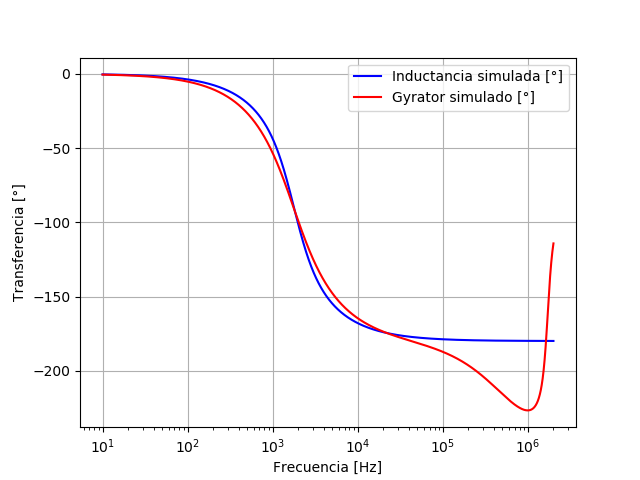
\includegraphics[width=0.7\textwidth]{ImagenesEj2/simLPP.PNG}
	\caption{Comparación de modelos Gyrator e Inductor Fase.}
	\label{fig:gyrIndPL}
\end{figure}
%%
\subsubsection{Elección de componentes.}
Se eligieron los componentes teniendo en cuenta la tabla (\ref{tab:specs}) para la cual el filtro debe cumplir esas especificaciones.
Lo primero que se decidió fue fijar la impedancia de salida del Gyrator siendo esta de $L \approx 10mH $ y $r_{coil} \approx 51\Omega $, para esto se tomaron los siguientes valores: $R_L = 51\Omega \ R_g = 200k\Omega \ C_g = 1nF$
A partir de esto se decidio una frecuencia de corte de  para que cumpla las especificaciones $f_c =1.78kHz $. Esto define un valor de capacitor $C \approx 800nF$ y finalmente dado a que no debe amplificar para ninguna frecuencia se eligió un valor de R tal que no haya sobrepico\footnote{Cabe aclarar que el valor de $\xi$ para el cual comienza a haber sobrepico es de 0.707} teniendo un valor de $\xi \approx 0.8 $ con $R \approx 130 $ y teniendo en cuenta la $r_{coil} = 51\Omega$  
Vale la pena notar que las aproximaciones que se expresaron en (\ref{eq:basicL2}) siguen vigentes. En este caso se tienen los siguientes valores:
\begin{align}  R<<R_g \implies  \frac{R_g}{R}=  1538 \ \ \ \ C_gR_L << 1 \implies C_gR_L =5.1\cdot 10^{-8} \end{align}


%%
\subsubsection{Respuesta en frecuencia.}
Se midió la respuesta en frencuencia del filtro pasa altos, se simuló en \textbf{LTSpice}  tanto el comportamiento con gyrator como el de un inductor. Obteniendo las siguientes gráficas:
\begin{figure}[H]	
	\centering
	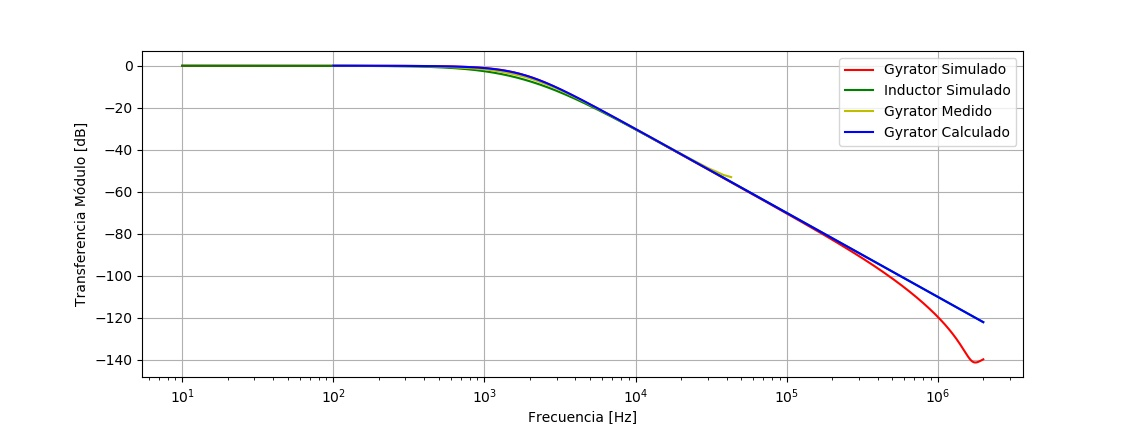
\includegraphics[width=\textwidth]{ImagenesEj2/bodelp.jpg}
	\caption{Diagrama BODE Low-Pass Amplitud.}
	\label{fig:bodelp}
\end{figure}
\begin{figure}[H]	
	\centering
	
\includegraphics[width=\textwidth]{ImagenesEj2/bodelpp.jpg}
	\caption{Diagrama BODE Low-Pass Fase.}
	\label{fig:bodelpp}
\end{figure}
Se puede observar que...
%%
\subsubsection{Analisis de resultados.}
El mayor interés fue puesto en que el circuito cumpla con las especificaciones dadas en la tabla (\ref{tab:specs})
Obteniendo las siguientes mediciones:


En la figura (\ref{fig:fahp}) se puede observar como para frecuencias a partir de 3kHz la atenuación es mayor a 12dB.
\begin{figure}[H]	
	\centering
	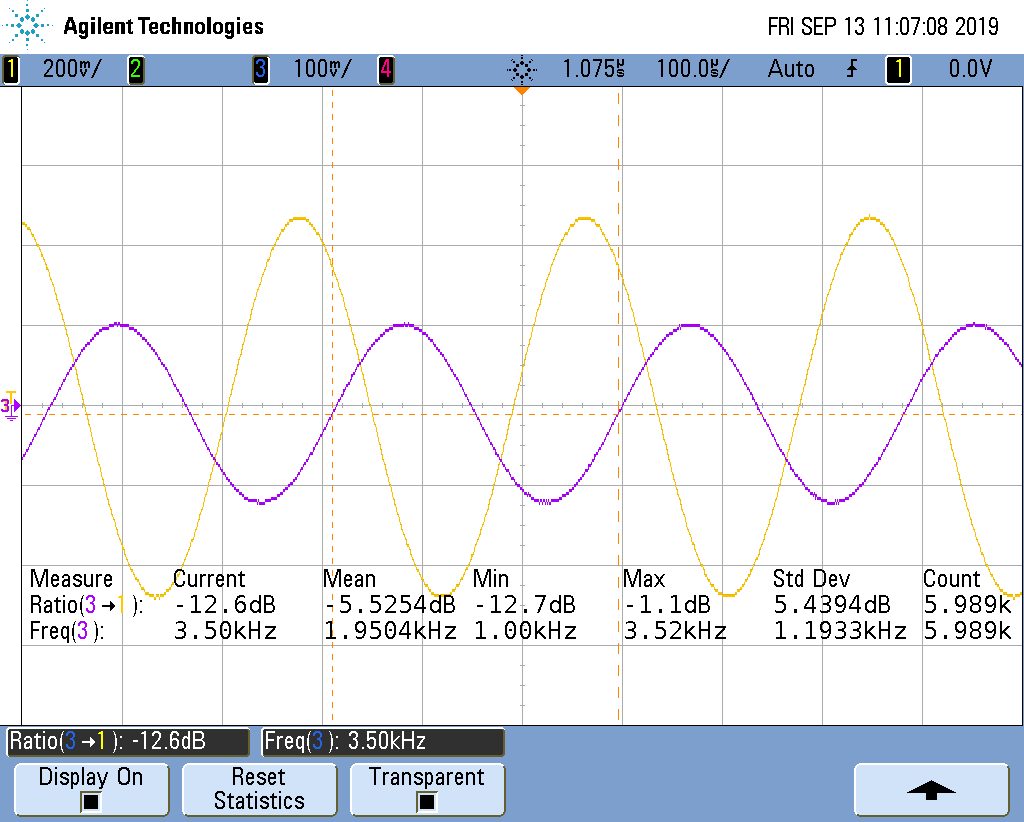
\includegraphics[width=\textwidth]{ImagenesEj2/MedicionesGrilla/fa_lp.png}
	\caption{Frecuencia de atenuación.}
	\label{fig:falp}
\end{figure}

En la figura (\ref{fig:fphp}) se puede observar como para frecuencias a partir de 10.5kHz, la atenuación es menor a 1.5dB.

\begin{figure}[H]	
	\centering
	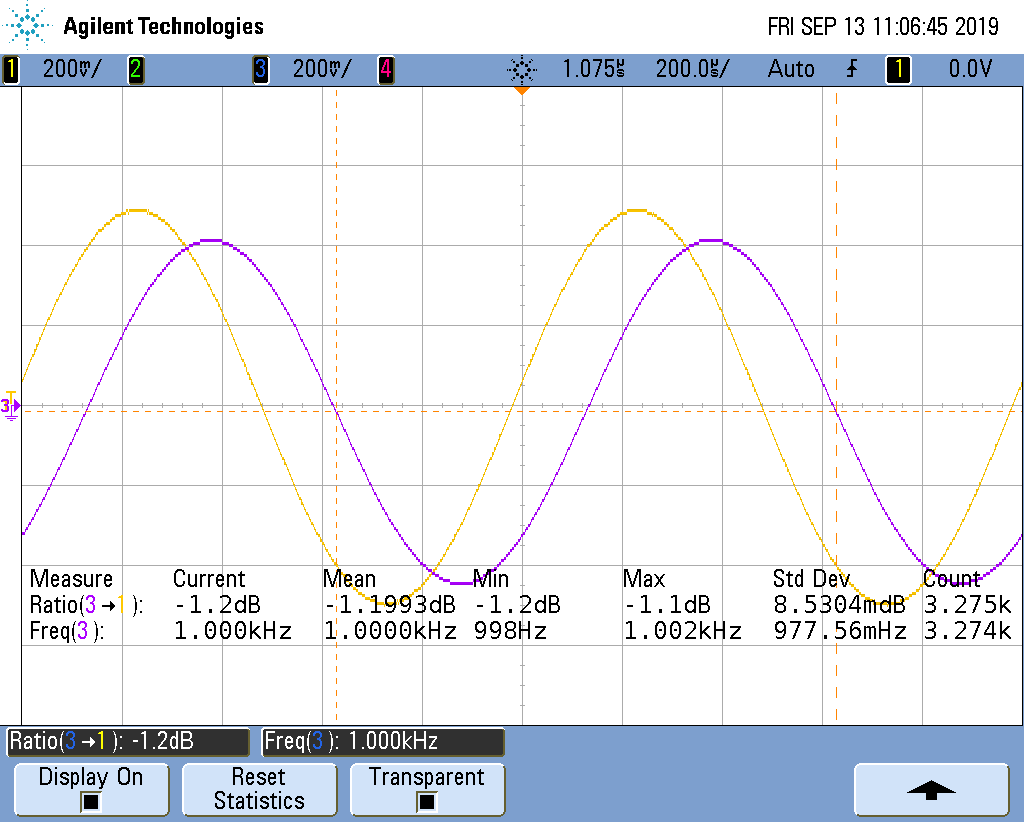
\includegraphics[width=\textwidth]{ImagenesEj2/MedicionesGrilla/fp_lp.png}
	\caption{Frecuencia de paso.}
	\label{fig:fplp}
\end{figure}
\newpage
%%%%%%%%%%%%%%%%%%%%%%%%%%%%%%%%%%%%%%%%%%%%
\subsection{Band Pass.}
\subsubsection{Circuito utilizando inductor.}
El circuito propuesto para realizar un filtro pasa banda clasicamente es el siguiente:

\begin{figure}[H]
\begin{center}
\begin{circuitikz}
	\node [](v2){};
	\draw (v2) node[label=left:$V_{In}$]{} to[short, o-] ++ (0.5,0) to[R, l = $R$]++ (2.5,0)  to[open] ++(0,-2) node[ground](gnd){};
	\draw (gnd) to[C, l_= $C$] ++(0,2);
	\draw(5,-2) node[ground](gnd2){};
	\draw (gnd2) to[L, l_= $L$] ++(0,2);

	\draw (v2) to[open] ++(3,0) to[short, -o] ++(3,0) node[label=right:$V_o$](){};
	\end{circuitikz}
	\caption{Filtro Band-Pass básico.}
	\label{fig:basBP}
\end{center}
\end{figure}
Operando en el circuito se obtiene:
\begin{align}H(s)=\frac{s\cdot \frac{L}{R}+\frac{r_{coil}}{R}}{s^2 LC+s\cdot (Cr_{coil}+\frac{L}{R})+1+\frac{r_{coil}}{R}}
	\label{eq:BPL}
\end{align}
%\begin{align}\end{align}
%%
\subsubsection{Circuito utilizando Gyrator.}
El circuito propuesto para el filtro Band-Pass es identico a la figura (\ref{fig:basBP}) con la singularidad que intercambiaremos el inductor por un gyrator de la siguiente manera.
\begin{figure}[H]	
	\centering
	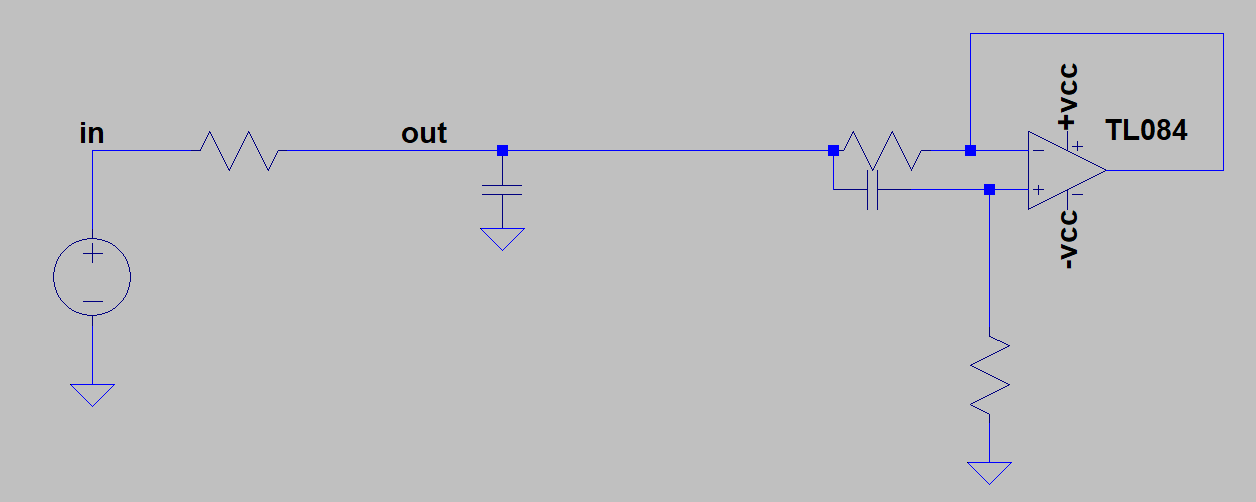
\includegraphics[width=0.7\textwidth]{ImagenesEj2/gyrBP.PNG}
	\caption{Filtro Band-Pass implementado con Gyrator.}
	\label{fig:gyrBP}
\end{figure}
Para resolver el circuito se plantearon la siguientes ecuaciones:
\begin{align}V^- = V_{o'}\end{align}
\begin{align}V_{o'} = A(s)\cdot (V^+-V^-)\end{align}
\begin{align} -\frac{V^+}{R_g}=(V^+-V_{out})\cdot sC_g \end{align}
\begin{align}  V_{out}\cdot sC= \frac{V^--V_{out}}{R_L}+\frac{V_{in}-V_{out}}{R}-\frac{V_{out}}{R_g+\frac{1}{sC_g}}\end{align}
Se llega a que:
\begin{align}H(s)=\frac{R_{L} \left(C_{g} R_{g} s + 1\right)}{C C_{g} R R_{L} R_{g} s^{2} + C R R_{L} s + C_{g} R R_{L} s + C_{g} R_{L} R_{g} s + R + R_{L}}
\end{align}
Teniendo en cuenta (\ref{eq:basicL1}) y (\ref{eq:basicL2}) se obtiene:
\begin{align}H(s)=\frac{s\frac{L}{R}+\frac{r_{coil}}{R}}{s^2\cdot LC +s \cdot (Cr_{coil}+\frac{L}{R})+1+\frac{r_{coil}}{R}}
\label{eq:BPG}
\end{align}
Vale la pena destacar que (\ref{eq:BPL}) y (\ref{eq:BPG}) son iguales.
%%
\subsubsection{Comparación de modelos.}
Se simuló en \textbf{LTSpice} ambos filtros, siendo estos el implemetnado con gyrator y el implementado con un inductor, obteniendo una coincidencia en todo el espectro a analizar, teniendo unas pequeñas diferencias para las tensiones que tienden a la continua.
\begin{figure}[H]	
	\centering
	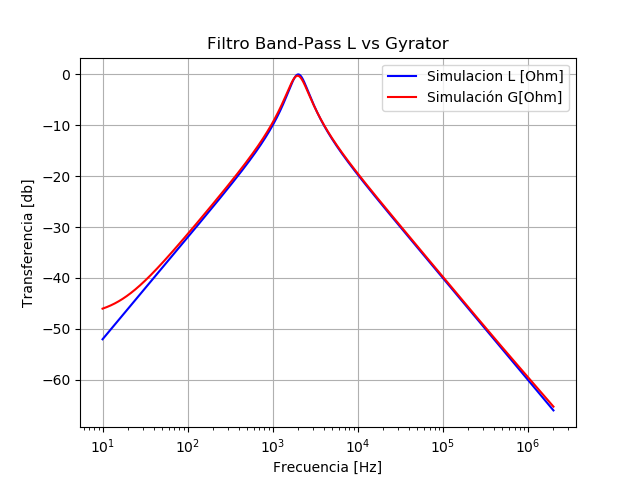
\includegraphics[width=0.7\textwidth]{ImagenesEj2/simBP.PNG}
	\caption{Comparación de modelos Gyrator e Inductor.}
	\label{fig:gyrIndBP}
\end{figure}
\begin{figure}[H]	
	\centering
	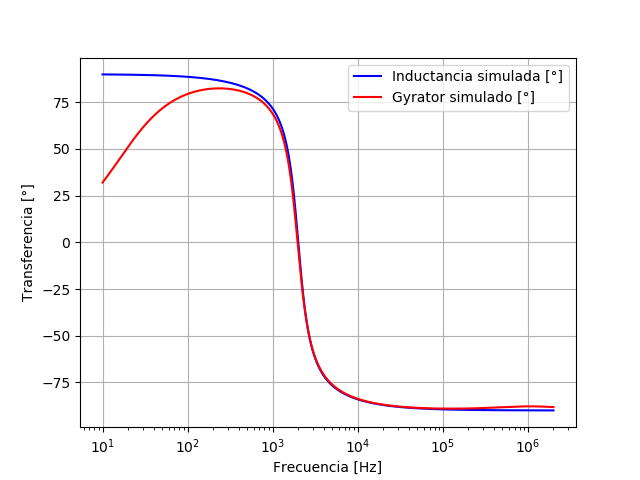
\includegraphics[width=0.7\textwidth]{ImagenesEj2/simBPP.PNG}
	\caption{Comparación de modelos Gyrator e Inductor Fase.}
	\label{fig:gyrIndPBP}
\end{figure}
%%

\subsubsection{Elección de componentes.}
Se eligieron los componentes teniendo en cuenta la tabla (\ref{tab:specs}) para la cual el filtro debe cumplir esas especificaciones.
Lo primero que se decidió fue fijar la impedancia de salida del Gyrator siendo esta de $L \approx 0.51H $ y $r_{coil} \approx 51\Omega $, para esto se tomaron los siguientes valores: $R_L = 51\Omega \ R_g = 1M\Omega \ C_g = 10nF$
A partir de esto se decidio una frecuencia de corte de  para que cumpla las especificaciones $f_c =2kHz $. Esto define un valor de capacitor $C \approx 800nF$ y finalmente dado a que no debe amplificar para ninguna frecuencia se eligió un valor de R tal que no haya sobrepico\footnote{Cabe aclarar que el valor de $\xi$ para el cual comienza a haber sobrepico es de 0.707} teniendo un valor de $\xi \approx 7.5 $ con $R \approx 12k\Omega $ y teniendo en cuenta la $r_{coil} = 51\Omega$  
Vale la pena notar que las aproximaciones que se expresaron en (\ref{eq:basicL2}) siguen vigentes. En este caso se tienen los siguientes valores:
\begin{align}  R<<R_g \implies  \frac{R_g}{R}=  84 \ \ \ \ C_gR_L << 1 \implies C_gR_Ls =5.1\cdot 10^{-7}\end{align}



%%
\subsubsection{Respuesta en frecuencia.}
Se midió la respuesta en frencuencia del filtro pasa altos, se simuló en \textbf{LTSpice}  tanto el comportamiento con gyrator como el de un inductor. Obteniendo las siguientes gráficas:
\begin{figure}[H]	
	\centering
	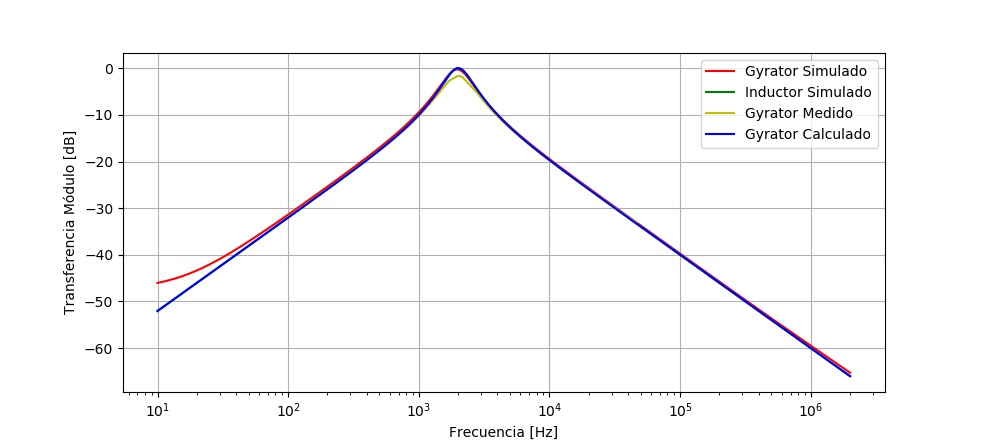
\includegraphics[width=\textwidth]{ImagenesEj2/bodebp.jpg}
	\caption{Diagrama BODE Band-Pass Amplitud.}
	\label{fig:bodebp}
\end{figure}
\begin{figure}[H]	
	\centering
	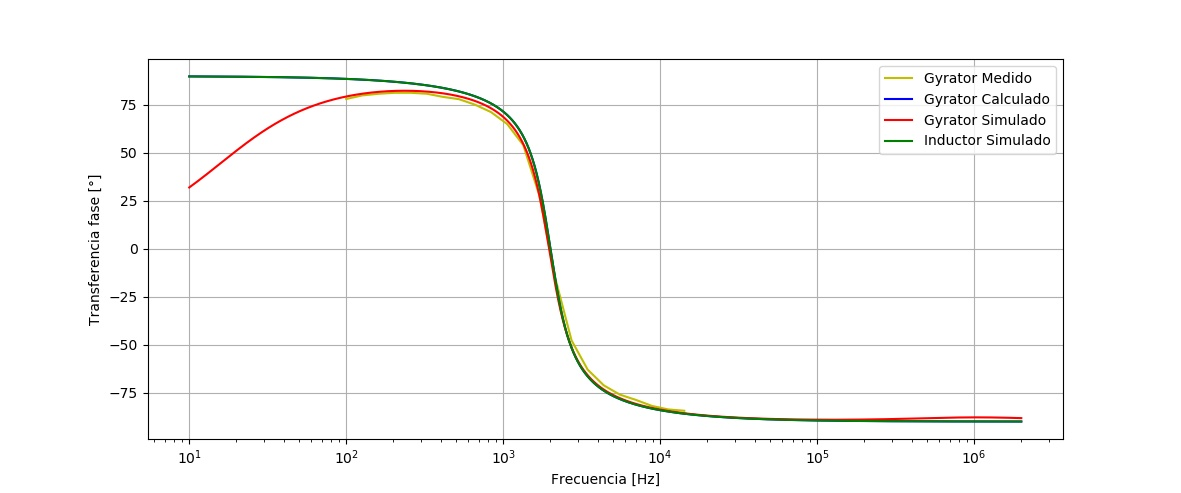
\includegraphics[width=\textwidth]{ImagenesEj2/bodebpp.jpg}
	\caption{Diagrama BODE Band-Pass Fase.}
	\label{fig:bodebpp}
\end{figure}
Se puede observar que...
%%

\subsubsection{Analisis de resultados.}
El mayor interés fue puesto en que el circuito cumpla con las especificaciones dadas en la tabla (\ref{tab:specs})
Obteniendo las siguientes mediciones:

En la figura (\ref{fig:fcbp}) se puede observar que para la frecuencias especificada en la tabla (\ref{tab:specs}) tendrá la minima atenuación.
\begin{figure}[H]	
	\centering
	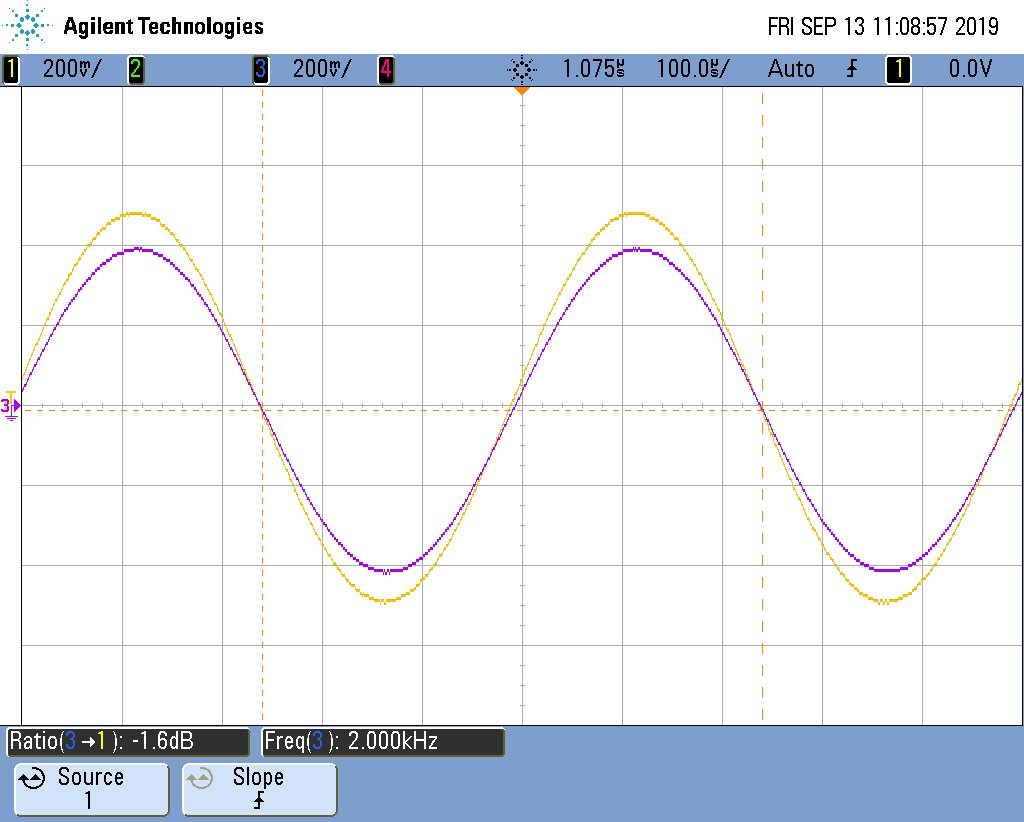
\includegraphics[width=\textwidth]{ImagenesEj2/MedicionesGrilla/fc_bp.png}
	\caption{Frecuencia de corte.}
	\label{fig:fcbp}
\end{figure}
\newpage
%%%%%%%%%%%%%%%%%%%%%%%%%%%%%%%%%%%%%%%%%%%%
\subsection{Band Reject.}
\subsubsection{Circuito utilizando inductor.}
El circuito propuesto para realizar un filtro rechaza banda clasicamente es el siguiente:
\begin{figure}[H]
\begin{center}
\begin{circuitikz}
	\node [](v2){};
	\draw (v2) node[label=left:$V_{In}$]{} to[short, o-] ++ (0.5,0) to[R, l = $R$]++ (1.5,0) to[L, l = $L$] ++ (0,-2) to[open](2,-4) node[ground](gnd){};
	\draw (gnd) to[C, l_= $C$] ++(0,2);
	\draw (v2) to[open] ++(2,0) to[short, -o] ++(1,0) node[label=right:$V_o$](){};
	\end{circuitikz}
	\caption{Filtro Band-Reject básico.}
	\label{fig:basBR}
\end{center}
\end{figure}
Al cual le corresponde una transferencia de la forma:
\begin{align} H(s)=\frac{s^2\cdot LC+s\cdot r_{coil}C+1}{s^2\cdot LC+s\cdot (RC+r_{coil}C)+1}
\label{eq:BRL}
\end{align}
%%
\subsubsection{Circuito utilizando Gyrator.}
\begin{figure}[H]	
	\centering
	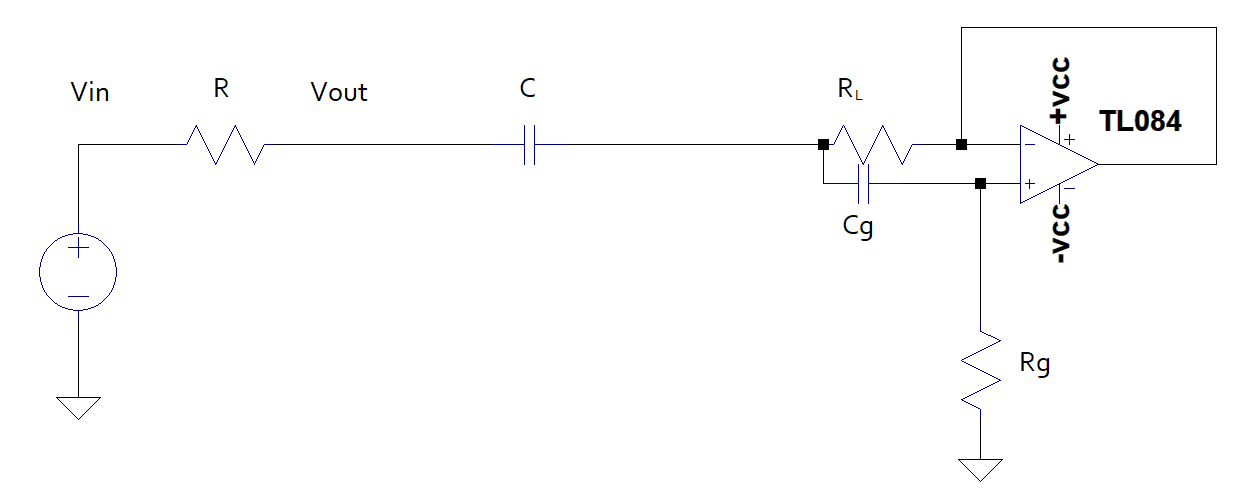
\includegraphics[width=0.7\textwidth]{ImagenesEj2/gyrBR.PNG}
	\caption{Filtro Band-Reject implementado con Gyrator.}
	\label{fig:gyrBR}
\end{figure}
Luego se procedió a analizar el circuito para sacar la función transferencia:
\begin{align}V^- = V_{o'}\end{align}
\begin{align}V_{o'} = A(s)\cdot (V^+-V^-)\end{align}
\begin{align}\frac{V_{out}-V_{in}}{R}=(V_n-V_{out})\cdot sC\end{align}
\begin{align}(V_n-V_{out})\cdot sC = \frac{-V_n}{R_g+\frac{1}{sC_g}}+\frac{V^--V_n}{R_L}\end{align}
\begin{align}\frac{-V^+}{R_g}=(V^+-V_n)\cdot sC_g\end{align}
Se llega a :
\begin{align}  H(s)=\frac{C C_{g} R_{L} R_{g} s^{2} + C R_{L} s + C_{g} R_{L} s + 1}{C C_{g} R R_{L} s^{2} + C C_{g} R_{L} R_{g} s^{2} + C R s + C R_{L} s + C_{g} R_{L} s + 1} \end{align}
Teniendo en cuenta (\ref{eq:basicL1}) y (\ref{eq:basicL2}) se obtiene:
\begin{align}  H(s)=\frac{ s^{2}\cdot  LC + s \cdot  C r_{coil} + 1}{ s^{2}\cdot LC + s\cdot (C R+Cr_{coil}) + 1} 
\label{eq:BRG}
\end{align}
%%
\subsubsection{Comparación de modelos.}
Se simuló en \textbf{LTSpice} ambos filtros, siendo estos el implemetnado con gyrator y el implementado con un inductor, obteniendo como era esperado una gran coincidencia en las frecuencias bajas y medias, y finalmente difiriendo en las altas como se ve a continuación:
\begin{figure}[H]	
	\centering
	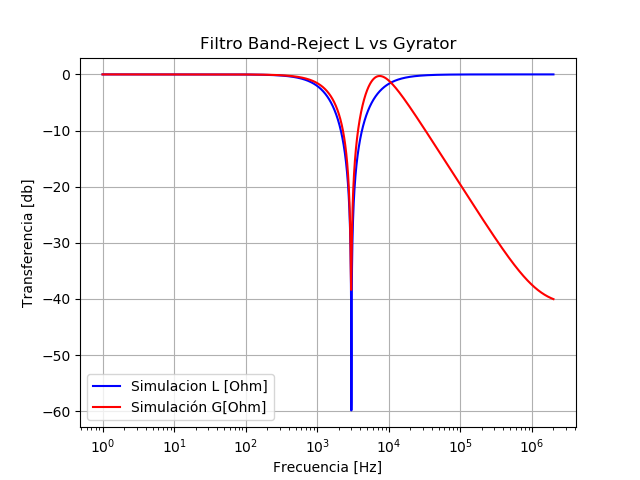
\includegraphics[width=0.7\textwidth]{ImagenesEj2/simBR.PNG}
	\caption{Comparación de modelos Gyrator e Inductor.}
	\label{fig:gyrIndBR}
\end{figure}
\begin{figure}[H]	
	\centering
	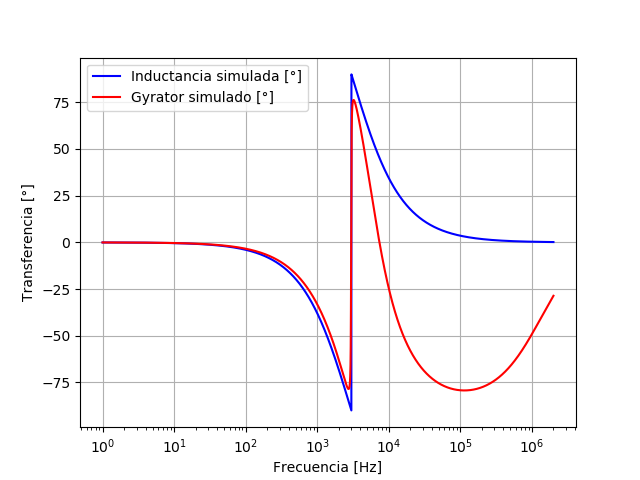
\includegraphics[width=0.7\textwidth]{ImagenesEj2/simBRP.PNG}
	\caption{Comparación de modelos Gyrator e Inductor Fase.}
	\label{fig:gyrIndPBR}
\end{figure}
%%
\subsubsection{Elección de componentes.}
Se eligieron los componentes teniendo en cuenta la tabla (\ref{tab:specs}) para la cual el filtro debe cumplir esas especificaciones.
Lo primero que se decidió fue fijar la impedancia de salida del Gyrator siendo esta de $L \approx 0.51H $ y $r_{coil} \approx 51\Omega $, para esto se tomaron los siguientes valores: $R_L = 51\Omega \ R_g = 1M\Omega \ C_g = 10nF$.
 Esto define un valor de capacitor $C \approx 4.7nF$ y finalmente dado a que no debe amplificar para ninguna frecuencia se eligió un valor de R tal que no haya sobrepico\footnote{Cabe aclarar que el valor de $\xi$ para el cual comienza a haber sobrepico es de 0.707} teniendo un valor de $\xi \approx 0.96 $ con $R \approx 20k\Omega $ y teniendo en cuenta la $r_{coil} = 51\Omega$  

Vale la pena notar que las aproximaciones que se expresaron en (\ref{eq:basicL2}) siguen vigentes. En este caso se tienen los siguientes valores:
\begin{align}  R<<R_g \implies  \frac{R_g}{R}=  50 \ \ \ \ C_gR_L << 1 \implies C_gR_L =5.1 \cdot 10^{-7} \end{align}

%%
\subsubsection{Respuesta en frecuencia.}

Se midió la respuesta en frencuencia del filtro pasa altos, se simuló en \textbf{LTSpice}  tanto el comportamiento con gyrator como el de un inductor. Obteniendo las siguientes gráficas:
\begin{figure}[H]	
	\centering
	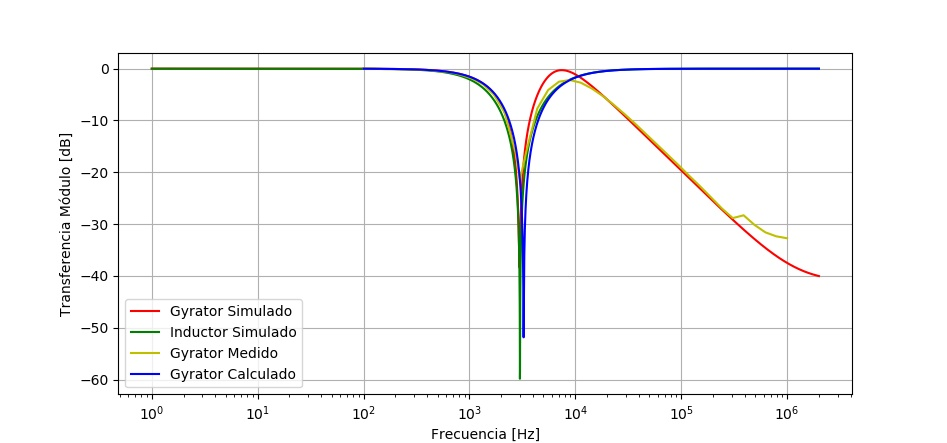
\includegraphics[width=\textwidth]{ImagenesEj2/bodebr.jpg}
	\caption{Diagrama BODE Band-Reject Amplitud.}
	\label{fig:bodebr}
\end{figure}
\begin{figure}[H]	
	\centering
	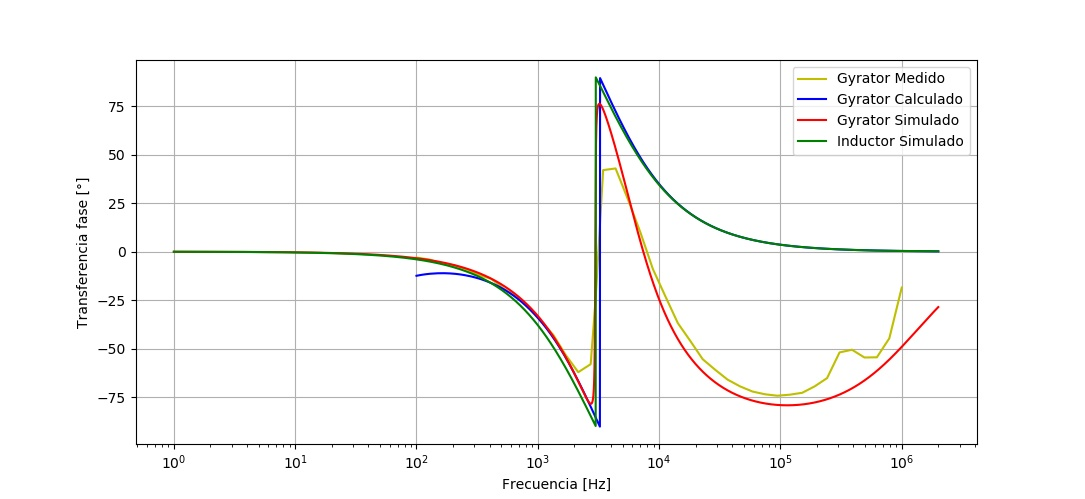
\includegraphics[width=\textwidth]{ImagenesEj2/bodebrp.jpg}
	\caption{Diagrama BODE Band-Reject Fase.}
	\label{fig:bodebrp}
\end{figure}
Se puede observar que...
%%
\subsubsection{Analisis de resultados.}

El mayor interés fue puesto en que el circuito cumpla con las especificaciones dadas en la tabla (\ref{tab:specs})
Obteniendo las siguientes mediciones:

En la figura (\ref{fig:fcbr}) se puede observar que para la frecuencias especificada en la tabla (\ref{tab:specs}) tendrá la máxima atenuación.
\begin{figure}[H]	
	\centering
	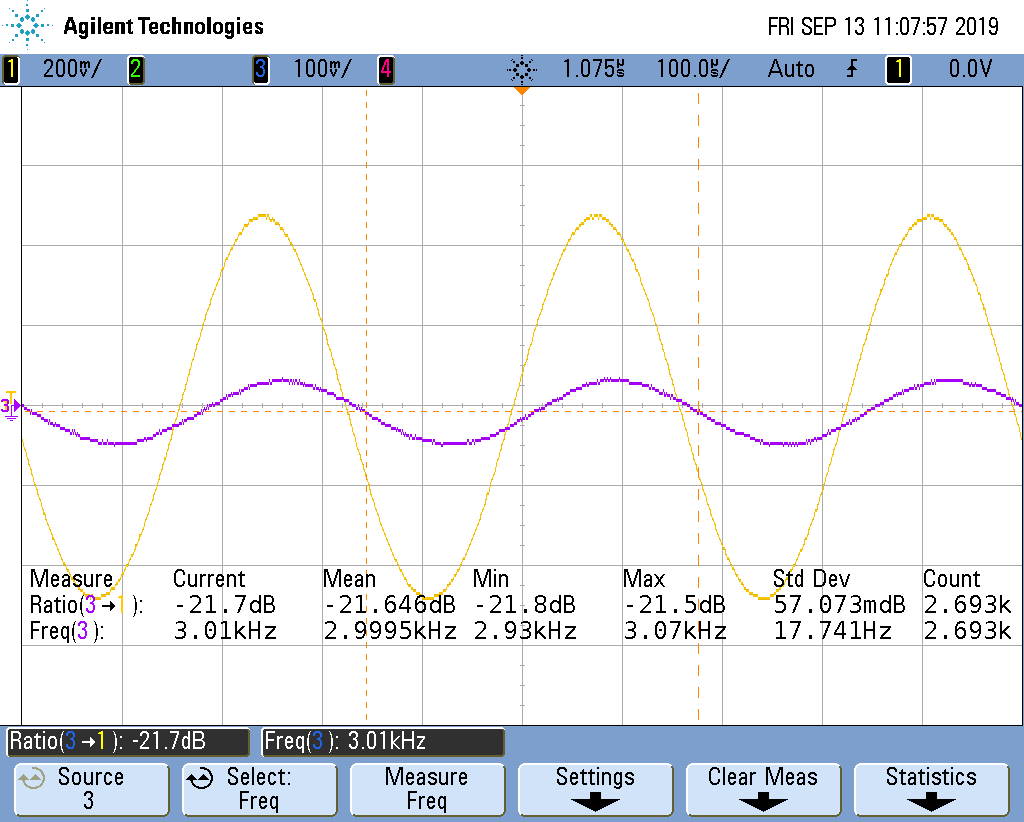
\includegraphics[width=\textwidth]{ImagenesEj2/MedicionesGrilla/fc_br.png}
	\caption{Frecuencia de corte.}
	\label{fig:fcbr}
\end{figure}
\newpage
%%%%%%%%%%%%%%%%%%%%%%%%%%%%%%%%%%%%%%%%%%%%
\subsection{Diseño en PCB.}
El circuito se diseño en el software \textbf{Altium Designer} dado a las condiciones de diseño requeridas, se optó por utilizar componentes \textbf{SMD} dado a que tienen un menor error y puede mantener mas acotado el tamaño final de la placa.
Se eligio utilizar un integrado TL084 utilizando cada opamp del mismo  para cada filtro y se pusieron capacitores de desacople para el mismo. Se obtuvo el siguiente esquemático:
\begin{figure}[H]	
	\centering
	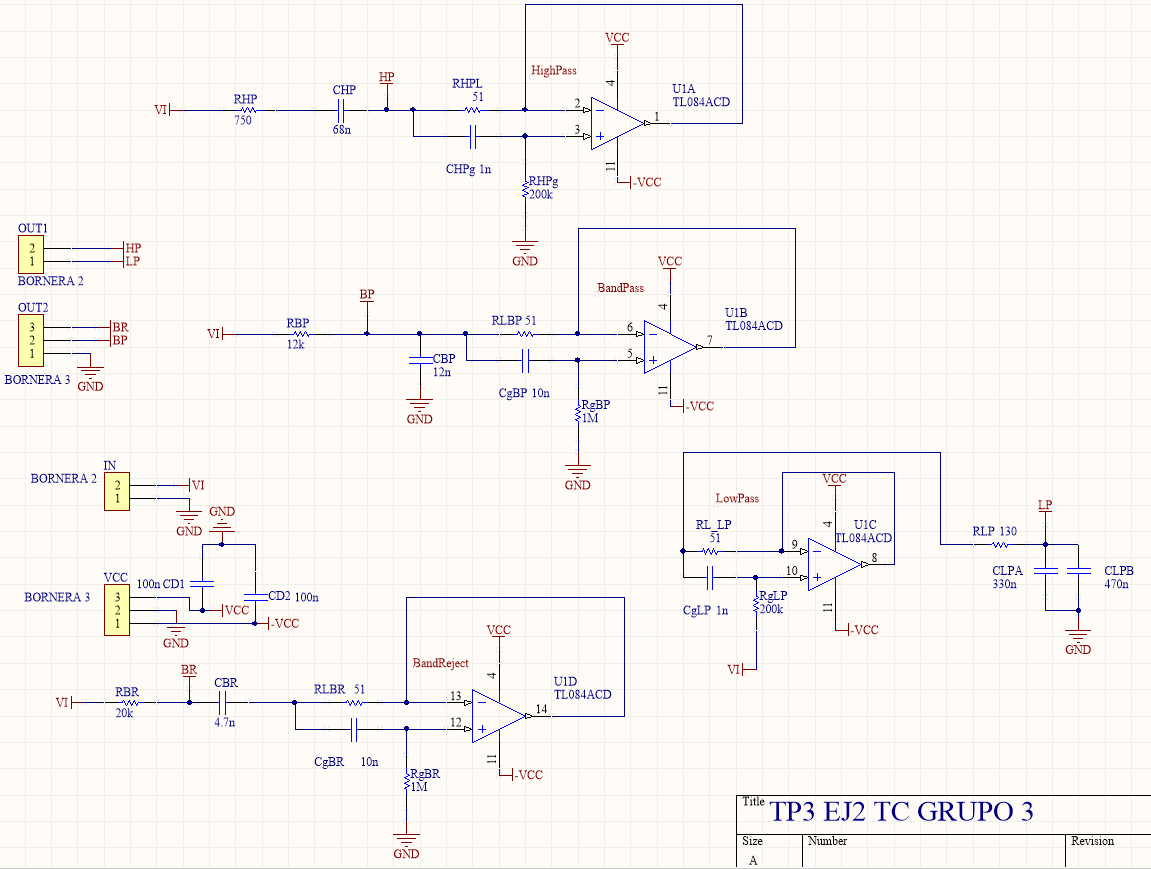
\includegraphics[width=\textwidth]{ImagenesEj2/esquematico.PNG}
	\caption{Esquemático del circuito.}
	\label{fig:esq}
\end{figure}
Luego se diseño el circuito en el PCB, se eligió utilizar una placa doble faz, dado a que al elegir utilizar componentes SMD y que tambien se deseaba que todos los componentes estén de un lado único no quedó otra opción.
\begin{figure}[H]	
	\centering
	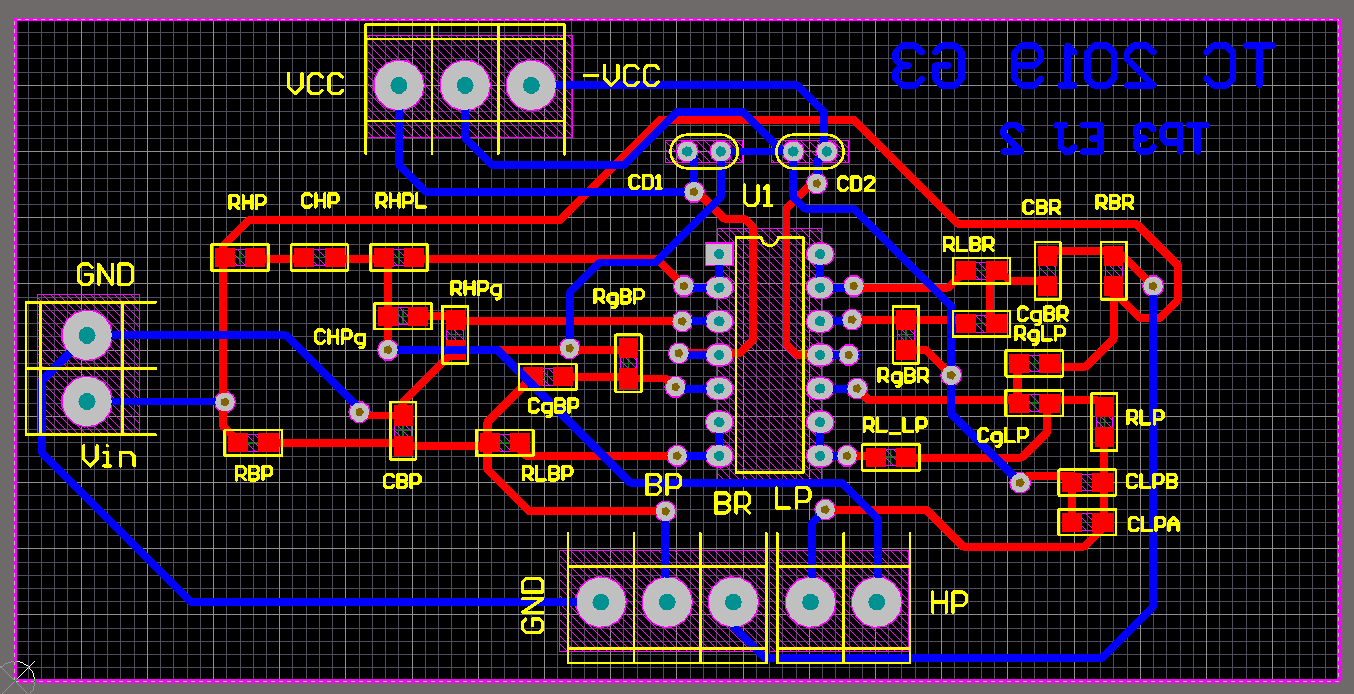
\includegraphics[width=\textwidth]{ImagenesEj2/pcb.PNG}
	\caption{PCB del circuito.}
	\label{fig:pcb}
\end{figure}
\end{document}
%\begin{align}\end{align}